\documentclass[convert={density=300,outext=.png}]{standalone}
\usepackage{tikz}
\usetikzlibrary{shapes,arrows,decorations,decorations.pathmorphing,arrows.meta,patterns,decorations.markings}

\begin{document}
%% Use \usepackage{tikz}
%% Use \usetikzlibrary{shapes,arrows,decorations, decorations.pathmorphing,arrows.meta,patterns}
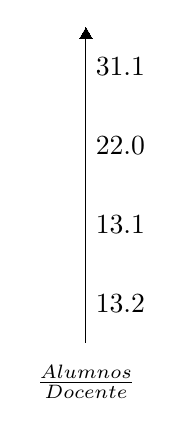
\begin{tikzpicture}[scale=1.0000]
	\tikzstyle{every node}=[scale=1.0000]
	
	%%Created with tikzpy
	
	\draw [line width = 0.0000 , fill= red!10 ,]  (0.0000,0.0000,0.0000) -- (0.0000,1.0000,0.0000);
	\draw [line width = 0.0000 , fill= red!10 ,]  (0.0000,1.0000,0.0000) -- (0.0000,2.0000,0.0000);
	\draw [line width = 0.0000 , fill= red!10 ,]  (0.0000,2.0000,0.0000) -- (0.0000,3.0000,0.0000);
	\draw [-{triangle 60[scale=1.0000]} ,line width = 0.0000 , fill= red!10 ,]  (0.0000,3.0000,0.0000) -- (0.0000,4.0000,0.0000);
	\node [right ,align=right]  at (0.0000,0.5000,0.0000)  {13.2};
	\node [right ,align=right]  at (0.0000,1.5000,0.0000)  {13.1};
	\node [right ,align=right]  at (0.0000,2.5000,0.0000)  {22.0};
	\node [right ,align=right]  at (0.0000,3.5000,0.0000)  {31.1};
	\node [align=center]  at (0.0000,-0.5000,0.0000)  {\textbf{$\frac{Alumnos}{Docente}$}};

\end{tikzpicture}
\end{document}
